\chapter{Background Tecnico}
\label{sec:background}


L'obiettivo di questo capitolo è presentare i concetti fondamentali dei sistemi eterogenei e della programmazione GPU, con particolare attenzione ai framework CUDA e Vulkan. Ottenere una visione approfondita di tali concetti contribuirà a una migliore la comprensione delle scelte tecnologiche e dei dettagli implementativi discussi nel capitolo del progetto finale. 

Il capitolo è diviso in due sezioni: la prima si concentra sul modello di programmazione GPGPU, mentre la seconda fornirà un'analisi dettagliata di CUDA e Vulkan per lo sviluppo di software e verrà giustificata la scelta del linguaggio Rust per la programmazione con Vulkan.

\section[General-purpose computing su GPU]{General-purpose computing su GPU}

Sebbene CPU e GPU siano entrambi processori che eseguono istruzioni macchina, esse differiscono soprattutto nell'approccio usato nell'eseguire programmi paralleli: mentre le CPU multi-core possono adottare un approccio di tipo Multiple Instruction Multiple Data (\gls{MIMD}) o Single Instruction Multiple Data (\gls{SIMD}), le GPU seguono un modello di istruzioni di tipo Single Instruction Multiple Thread (\gls{SIMT}), in cui il carico di lavoro è suddiviso in sotto-problemi risolvibili da singoli thread indipendenti. Lo sviluppo delle GPU si è storicamente concentrato nell'ambito delle industria dei videogiochi, il cui l'impegno tecnologico è sempre stato finalizzato a offrire esperienze virtuali il più realistiche possibili. Per raggiungere questo obiettivo, sono richiesti un numero considerevole di calcoli geometrici (tipicamente rotazioni e traslazioni) per ogni pixel dello schermo, sotto forma di operazioni in virgola mobile. Le architetture delle GPU sono strutturate seguendo il modello many-thread anziché multi-core, mettendo quindi l'accento sull'ottimizzazione del trattamento dei dati piuttosto che sulla memorizzazione e sul controllo del flusso.
Entrambi i modelli sono rappresentati in fig. \ref{fig:cpu_vs_gpu}.

\begin{figure}[ht]
    \centering
    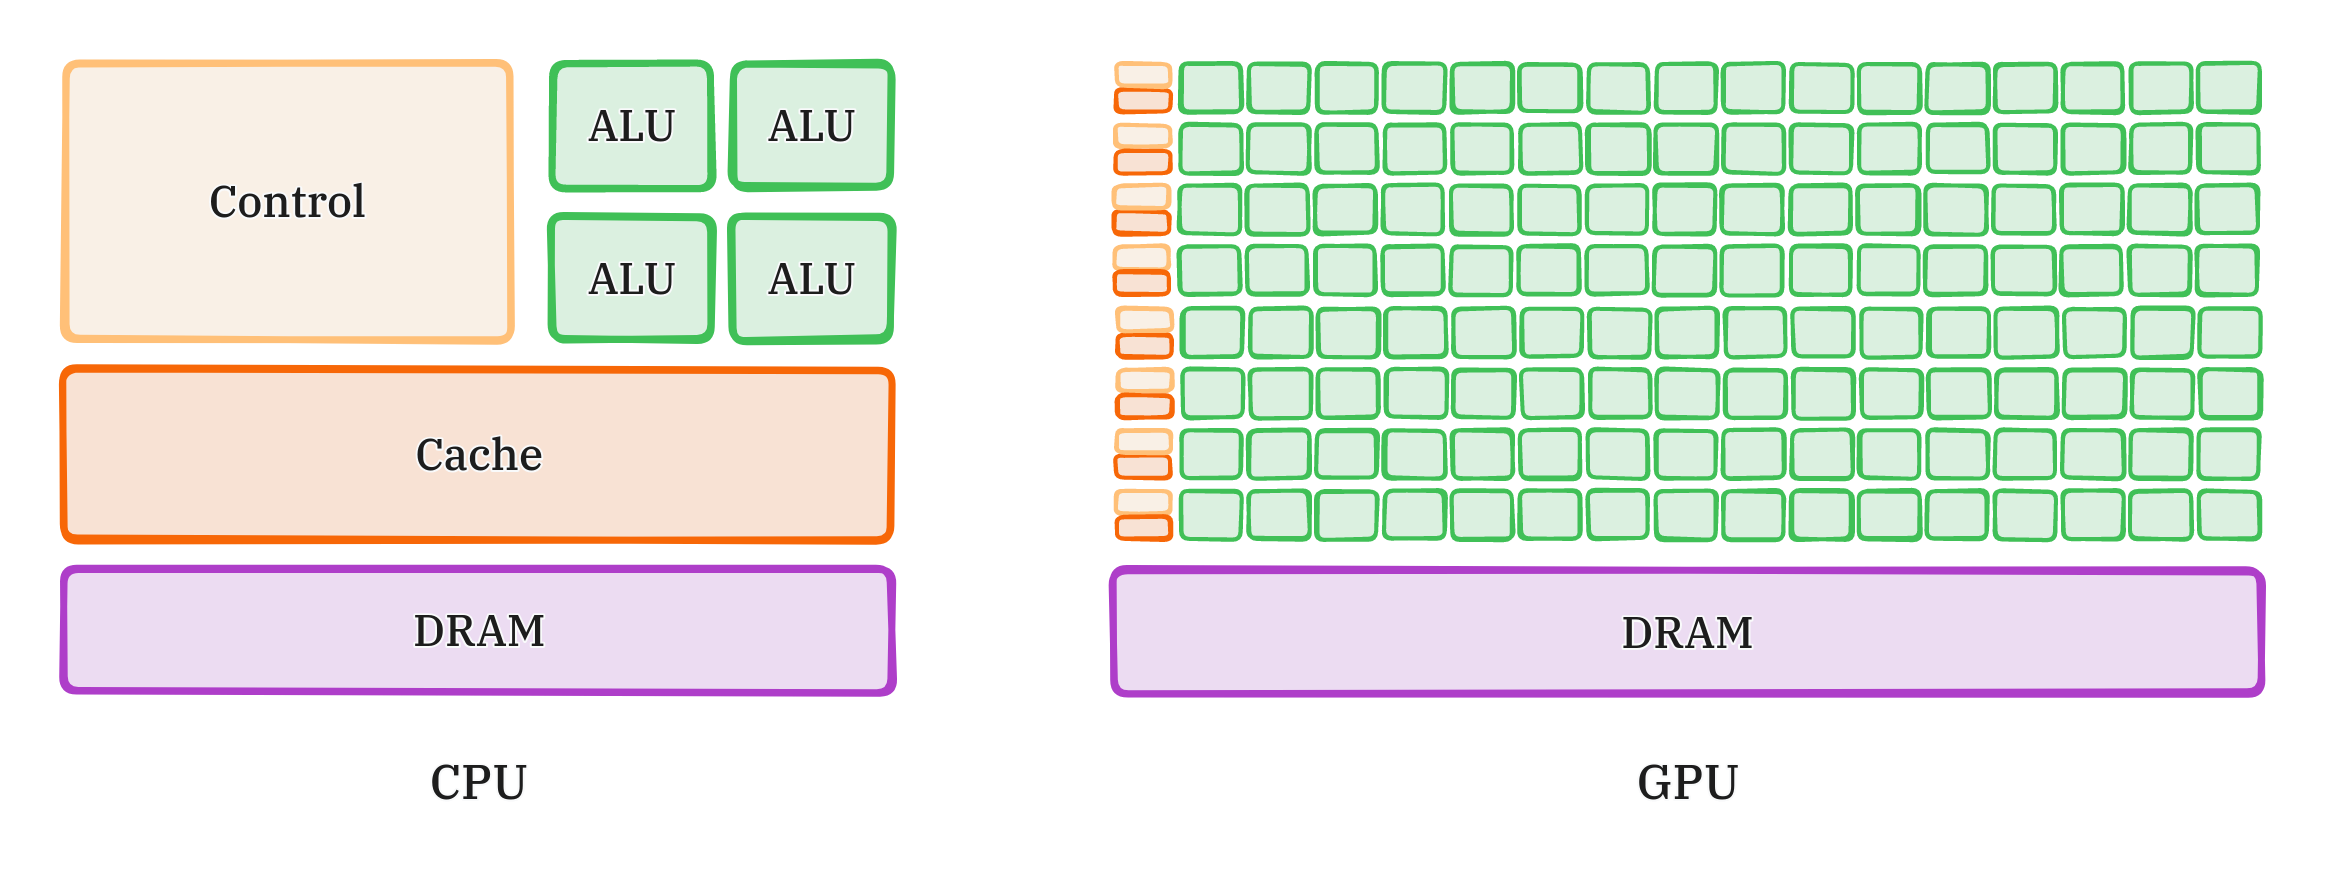
\includegraphics[width=.9\linewidth]{images/chapter2/cpu_vs_gpu.png}
    \caption{Confronto fra l'architettura CPU e GPU}
    \label{fig:cpu_vs_gpu}
\end{figure}

Il paradigma di GPGPU consente di sfruttare la potenza di calcolo delle GPU non solo per la grafica dei videogiochi, ma anche per eseguire calcoli generici di natura scientifica ed ingegneristica, come l'ottimizzazione nella simulazione di sistemi fisici reali. Grazie alla GPGPU, il trasferimento di dati tra CPU e GPU diventa bidirezionale e, di conseguenza, in sistemi che richiedono numerose operazioni su grandi quantità di dati, si può osservare un notevole miglioramento delle prestazioni. Un'implementazione intelligente del paradigma SIMD su GPU può conseguire un aumento di velocità fino a 100 volte rispetto a un'implementazione sequenziale su un singolo core CPU. Secondo la tassonomia di Flynn \cite[]{Flynn:tax}, un sistema è classificato come SIMD se esegue una singola istruzione, o anche un piccolo insieme di istruzioni, in parallelo su un vasto numero di dati. Il paradigma SIMT è simile, e affida l'esecuzione di un ristretto insieme di istruzioni a un singolo thread, sarà poi compito del programmatore aggregare i risultati di ogni thread GPU e ottenere il risultato finale della computazione.

In genere, un sistema non può essere parallelizzato in tutte le sue parti, limitando l'accelerazione delle prestazioni a una piccola porzione del codice. Pertanto, è necessario progettare sistemi in cui alcune parti siano concepite in parallelo, mentre altre in modo sequenziale. Per questo motivo, nel modello GPGPU, CPU e GPU collaborano tra loro, dando origine a un modello di elaborazione eterogenea in cui la CPU gestisce la parte sequenziale, mente la GPU esegue in parallelo la parte computazionalmente onerosa.
La fig. \ref{fig:het_model} mostra il modello di un sistema eterogeneo: il carico di lavoro parallelizzabile, è affidato alla GPU, mentre il compito di gestire i processi e la suddivisione in sotto-problemi è affidata alla CPU.

\begin{figure}[ht]
    \centering
    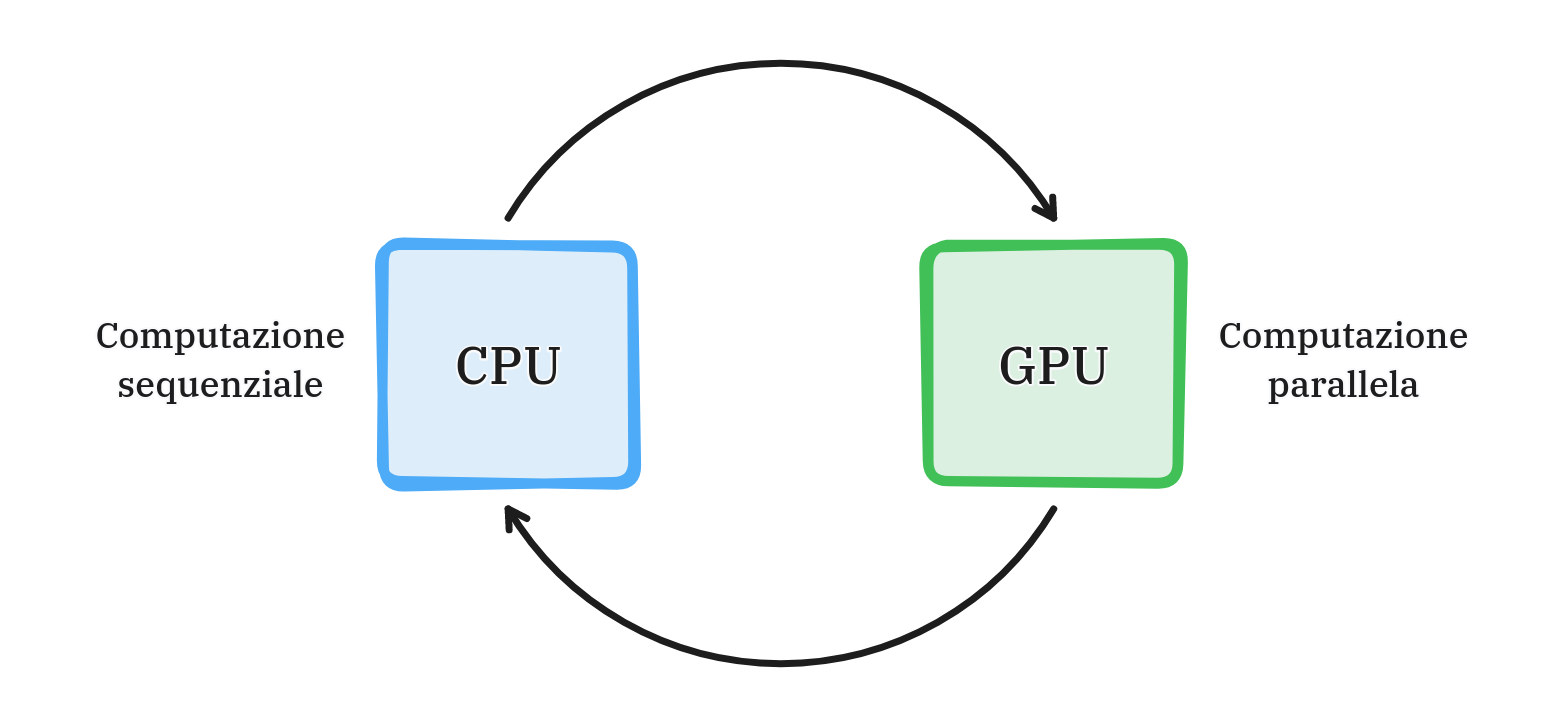
\includegraphics[width=.9\linewidth]{images/chapter2/het_model2.png}
    \caption{Modello di un sistema eterogeneo}
    \label{fig:het_model}
\end{figure}


Inizialmente, le GPU e i linguaggi di programmazione parallela erano destinati a un mercato molto diverso rispetto a quello delle CPU. Nella programmazione `classica' delle CPU, la compatibilità tra diverse versioni dello stesso software è stata fin dall'inizio un requisito fondamentale, mentre l'innovazione in termini di miglioramento delle GPU ha spesso comportato cambiamenti drastici nell'hardware. Queste evoluzioni tecnologiche hanno portato a una perdita di portabilità tra i diversi modelli: l'introduzione di nuove tecnologie hardware ha portato a proposte di architetture GPU completamente nuove, con significative differenze tra loro. Di conseguenza, queste nuove architetture richiedevano quasi sempre una ridefinizione completa dei relativi codici. Si è rilevato quindi necessario stabilire degli standard operativi per poter, quantomeno, mantenere un modello logico coerente tra le diverse architetture.
I principali standard per l'elaborazione parallela sono MPI, OpenMP.

\begin{itemize}
    \item \textbf{MPI}: progettato per sistemi di memoria distribuita, utilizzato in ambienti di HPC in cui più processori o nodi comunicano scambiandosi messaggi. Solitamente viene usato per l'architettura di supercomputer, nei quali migliaia di nodi sono connessi attraverso una rete dedicata. Ogni problema viene suddiviso in diversi sotto-problemi, ognuno dei quali è risolto da un nodo specifico. Questo modello è poco flessibile e oneroso di risorse e soprattutto una rete dedicata molto veloce che si possa far carico dei messaggi tra i nodi.
    \item \textbf{OpenMP}: offre un insieme di direttive del compilatore e routine di libreria per il multiprocessing su singole macchine a memoria condivisa, comunemente usato per parallelizzare cicli e altre regioni di codice per sfruttare i processori multi-core. Dato che il software deve essere eseguito sulla stessa macchina questo modello è relativamente più semplice del precedente, ma limitato dal punto di vista prestazionale.
\end{itemize}

\begin{figure}[ht]
    \centering
    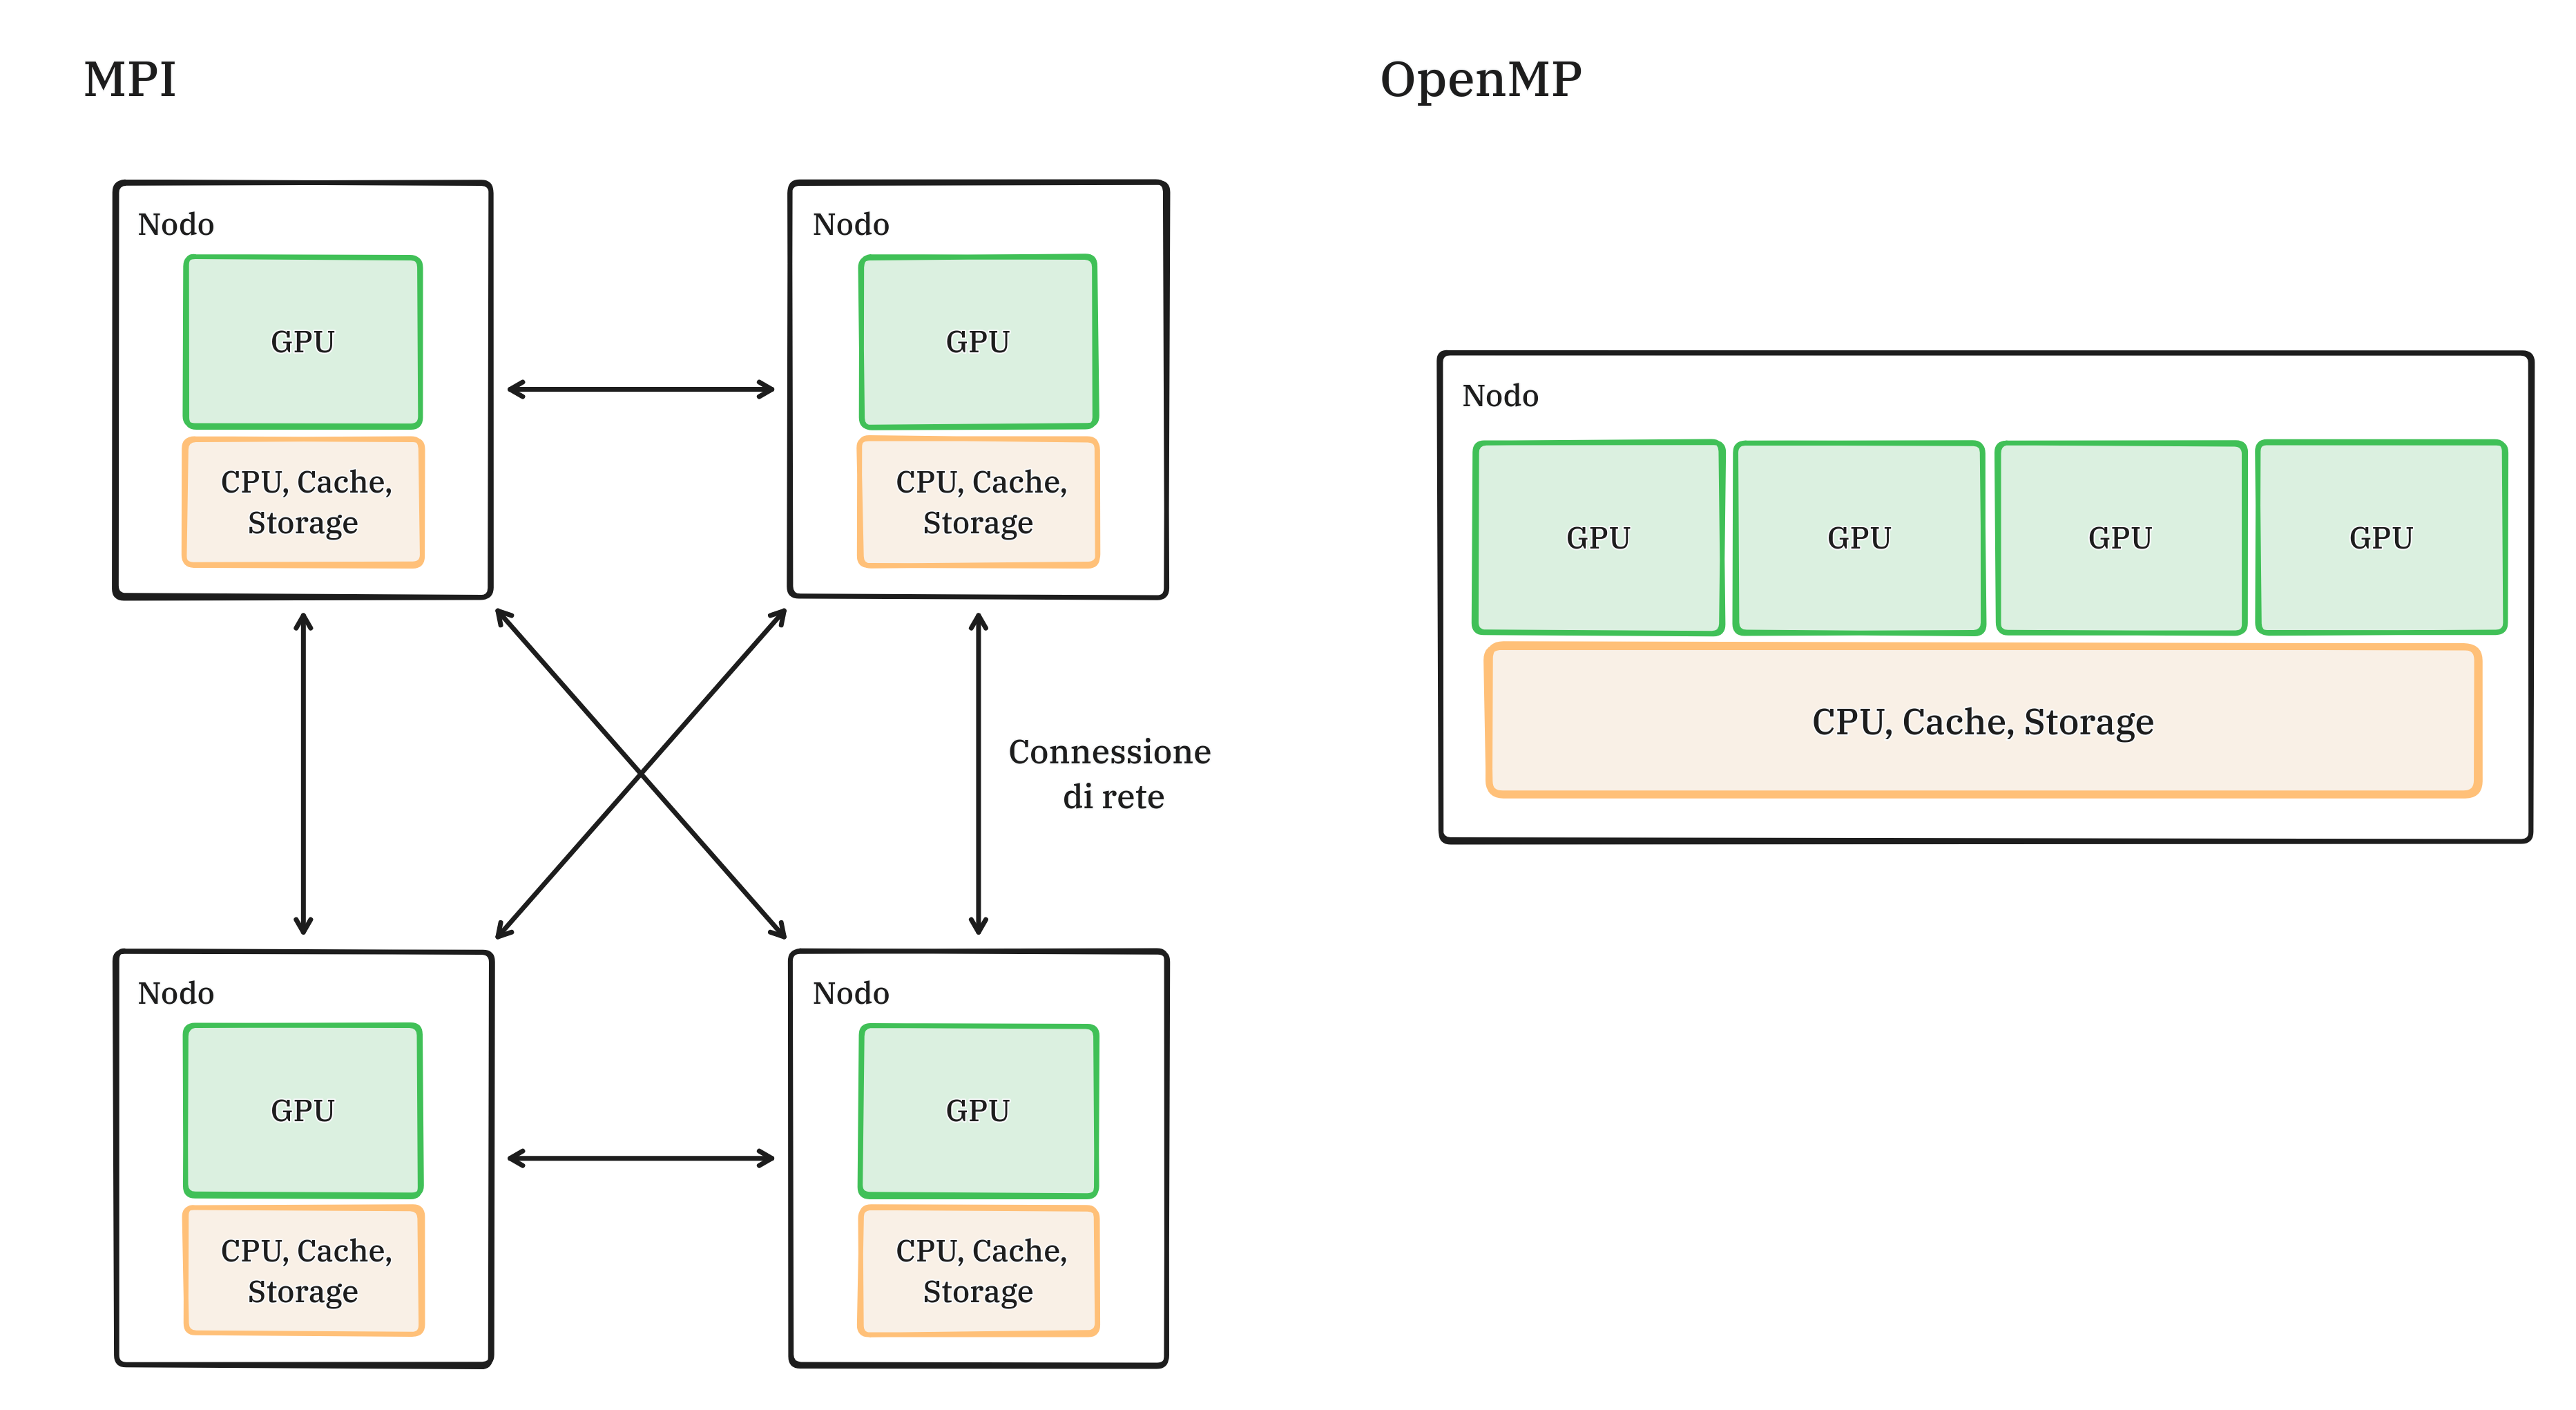
\includegraphics[width=.9\linewidth]{images/chapter2/mpi_openmp.png}
    \caption{Sistema MPI e OpenMP a confronto}
    \label{fig:mpi_openmp}
\end{figure}

Il modello OpenMP consente al programmatore di raggiungere un alto livello di parallelizzazione, specificando, in modo semplice, le porzioni specifiche del codice da ottimizzare. D'altra parte, in MPI i nodi non condividono la memoria e tutti i dati sono condivisi attraverso messaggi, garantendo elevata scalabilità anche su centinaia di miglia di nodi; implementarlo, però,  può risultare difficile proprio per la mancanza di memoria condivisa tra i nodi. A causa della loro natura intrinsecamente diversa, è raro utilizzare contemporaneamente questi standard. In fig. \ref{fig:mpi_openmp} è mostrata la sostanziale differenza tra i due modelli.

\begin{figure}[ht]
    \centering
    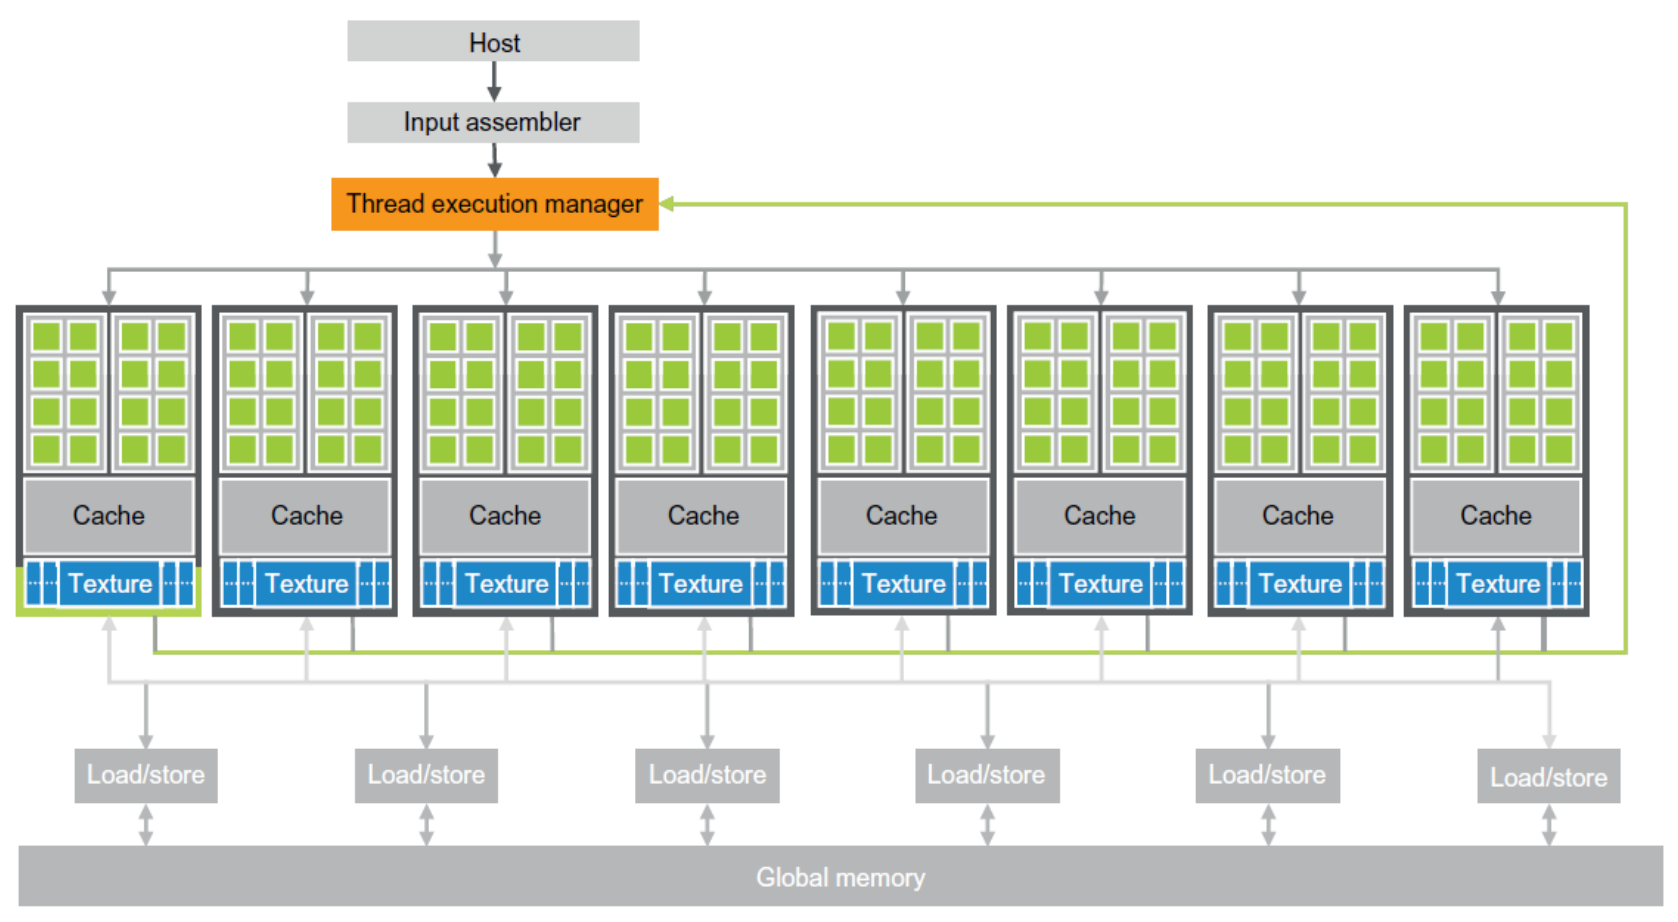
\includegraphics[width=.9\linewidth]{images/chapter2/cuda_arch.png}
    \caption{Architettura di una GPU CUDA-compatibile}
    \label{fig:cuda_arch}
\end{figure}

Con l'introduzione di CUDA, NVIDIA ha fornito agli sviluppatori un framework in grado di combinare i vantaggi dei due standard. Con l'acronimo CUDA, che sta per Compute Unified Device Architecture, si intende non solo il linguaggio di programmazione, ma anche l'architettura hardware. Per sfruttare questo framework, è necessaria una GPU compatibile con CUDA e, dato che è sviluppato da NVIDIA, tutte le loro GPU recenti lo supportano. L'architettura tipica di una GPU NVIDIA compatibile con CUDA è illustrata in fig. \ref{fig:cuda_arch}. Le differenze tra i vari modelli possono essere negli Streaming Multiprocessors (SMs) e nei Stream Processors (SPs), ma non ci si addentrerà ulteriormente in questo concetto. Ogni GPU recente è dotata di gigabyte di memoria dedicata denominata Graphics Double Data Rate \gls{GDDR}, un tipo di memoria SDRAM, usata per memorizzare temporaneamente informazioni necessarie alla computazione, evitando di doverle recuperare nella memoria centrale del sistema, operazione che richiederebbe più cicli di clock.


\section[Framework di programmazione su GPU]{Framework di programmazione su GPU}


Con il rilascio di CUDA, nel 2007, NVIDIA commercializza la prima GPU che riserva aree specifiche di silicio per semplificare la programmazione parallela. Questo non rappresenta solo cambiamenti software, ma vennero aggiunti nuovi componenti hardware ai chip stessi. Nei chip G80 e nei loro successori dedicati al calcolo parallelo, i programmi CUDA non attraversano più l'interfaccia grafica. Invece, una nuova interfaccia di programmazione parallela ad uso generale gestisce le richieste dei programmi CUDA. Questa interfaccia di programmazione espande notevolmente i tipi di applicazioni che è possibile sviluppare per le GPU. Inoltre, anche tutti gli altri strati software furono ridisegnati, consentendo ai programmatori di utilizzare i familiari strumenti di programmazione C/C++. Sebbene sia ancora possibile usare la vecchia interfaccia di programmazione basata su OpenGL, l'avvento di CUDA e il supporto al computing da parte di NVIDIA ha reso molto più semplice sviluppare applicazioni parallele eliminando la necessità di utilizzare API grafiche e di esprimere i calcoli sotto forma di funzioni che colorano un pixel.

Solamente un anno dopo Khronos Group, un consorzio industriale che gestisce lo sviluppo e la promozione di standard aperti, rilascia OpenCL, framework che fornisce una piattaforma aperta e standardizzata per la programmazione parallela su sistemi eterogenei. Così come CUDA, anche OpenCL mira a fornire una piattaforma unificata per lo sviluppo di applicazioni che possono sfruttare le capacità di elaborazione parallela, ma, a differenza di CUDA, OpenCL supporta varie architetture hardware e non ha bisogno di chip dedicati. Un aspetto fondamentale di OpenCL è la sua natura di standard aperto e multi-piattaforma: ciò significa che gli sviluppatori possono scrivere codice OpenCL che può essere eseguito su più dispositivi, indipendentemente dal produttore. OpenCL ha subito diverse revisioni nel corso degli anni per migliorare le funzionalità e la flessibilità. 

\begin{figure}[ht]
    \centering
    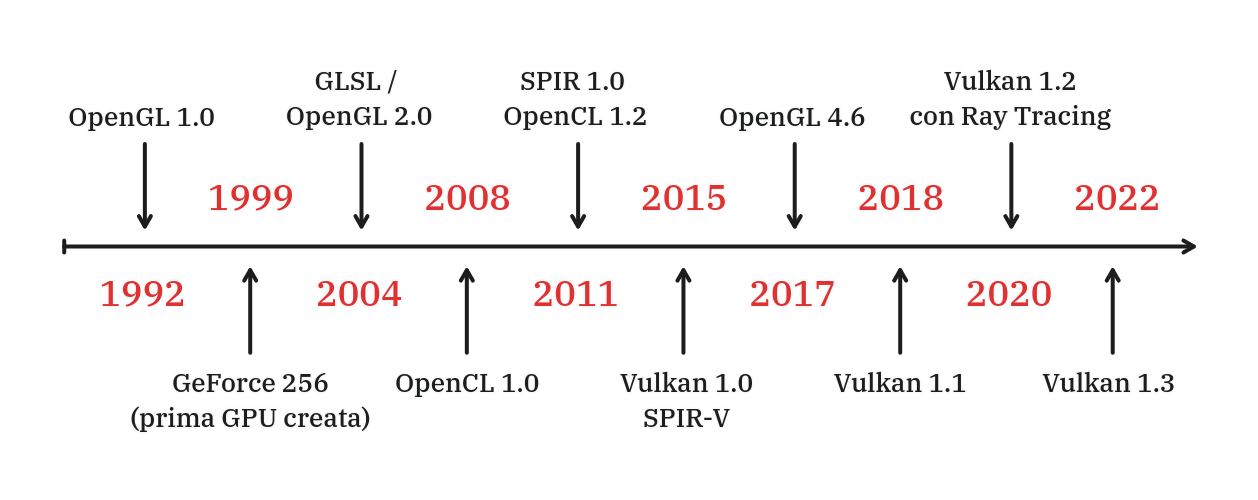
\includegraphics[width=.9\linewidth]{images/chapter2/vulkan_history.png}
    \caption{Contributi di Khronos Group}
    \label{fig:vulkan_history}
\end{figure}

Col tempo, Khronos Group ha riconosciuto la necessità di unire le caratteristiche di grafica e calcolo in un'unica API. Vulkan è stata sviluppata con l'obiettivo di superare le limitazioni di OpenGL e di fornire un accesso più diretto alle risorse hardware, consentendo una maggiore parallelizzazione e un maggiore controllo da parte degli sviluppatori. Vulkan offre una serie di funzionalità che lo rendono più efficiente e flessibile rispetto ad OpenGL e OpenCL, inclusa una migliore gestione delle risorse, un controllo più diretto sulla GPU, una maggiore parallelizzazione e un minore overhead dei driver. Vulkan è progettata per essere più adatta agli sviluppatori che richiedono il massimo delle prestazioni all'hardware, come nei giochi e nelle applicazioni di realtà virtuale. In sintesi, Vulkan rappresenta una diretta evoluzione di OpenGL e OpenCL, cercando di unire le migliori caratteristiche di entrambe per fornire un'API più potente, efficiente e adatta alle moderne architetture hardware. In fig. \ref{fig:vulkan_history} è visibile l'evoluzione nel tempo delle API rilasciate da Khronos Group. Sia OpenGL che OpenCL sopravvivono tutt'oggi per la loro semplicità nello sviluppo delle applicazioni e l'ampio supporto hardware, sebbene siano meno performanti rispetto a CUDA e Vulkan.

\subsection[CUDA]{CUDA}

La struttura di un programma CUDA riflette la coesistenza di un host (CPU) e uno o più device (GPU) nel computer. Ogni file sorgente CUDA può contenere sia codice host che codice device. Da questo punto di vista, si può considerare un qualsiasi programma C/C++ come un programma CUDA che contiene solo codice host. Le dichiarazioni di funzioni o dati per il device sono chiaramente contrassegnate con particolari keyword di CUDA. Il codice deve essere compilato da un compilatore che riconosce e comprende queste dichiarazioni aggiuntive: il compilatore CUDA ufficiale è NVCC (NVIDIA C Compiler) prodotto da NVIDIA.

\begin{figure}[ht]
    \centering
    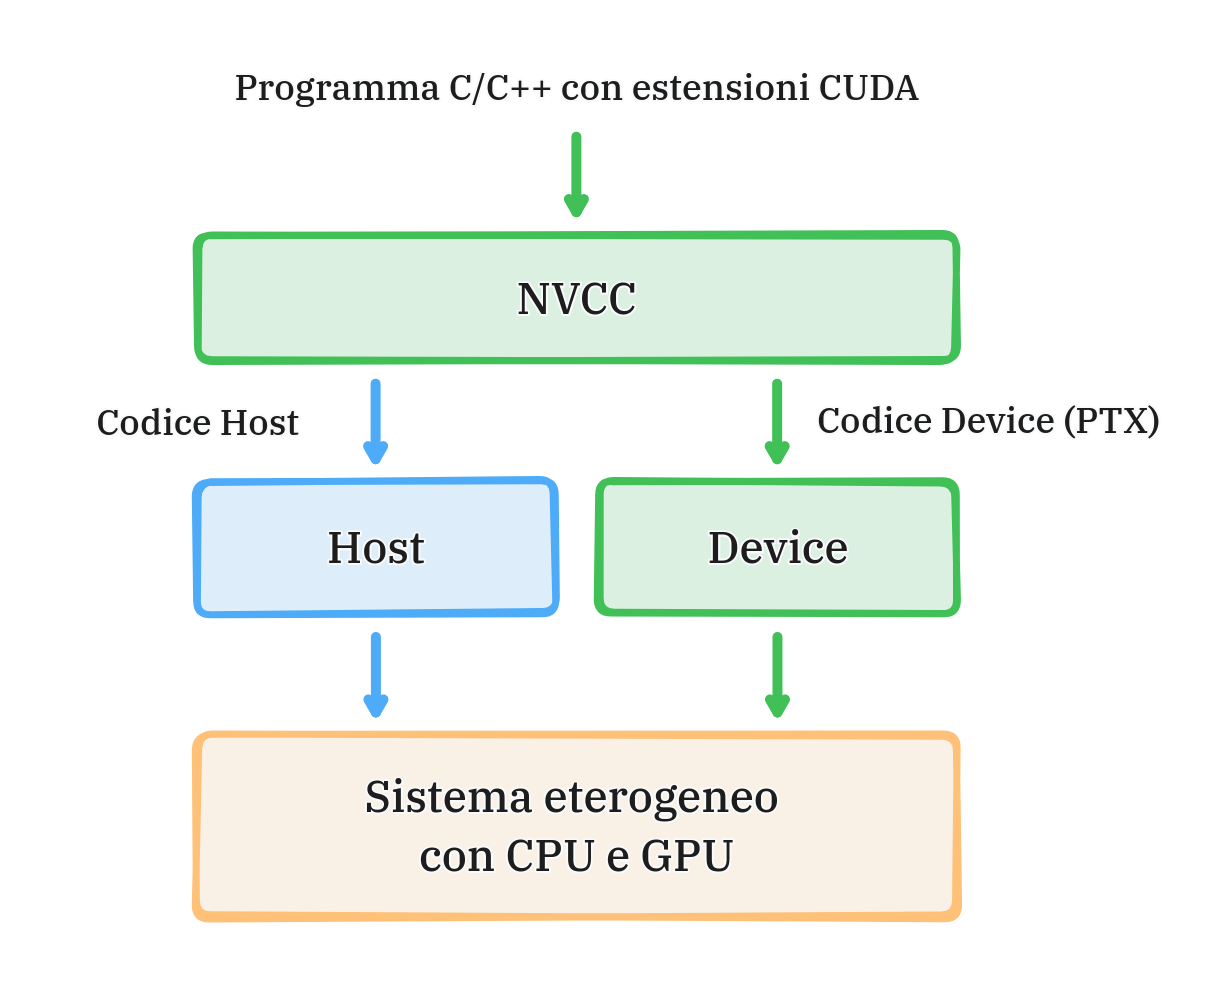
\includegraphics[width=.9\linewidth]{images/chapter2/nvcc.png}
    \caption{Processo di compilazione di un programma CUDA}
    \label{fig:nvcc}
\end{figure}

NVCC elabora il programma, utilizzando le keyword CUDA per separare il codice host e il codice device. Il codice host è normale codice ANSI C, che viene ulteriormente compilato dai compilatori standard C/C++ dell'host e viene eseguito come un processo CPU tradizionale. Il codice device è contrassegnato con le keyword CUDA \verb|__device__| o \verb|__global__| per etichettare le funzioni di parallelismo dei dati, chiamate kernel, e le relative strutture di dati associate. Il codice device viene ulteriormente compilato da un componente runtime di NVCC ed eseguito su un device GPU. L'esecuzione inizia sull'host e quando una funzione kernel viene chiamata, essa viene eseguita parallelamente dai thread del device. L'insieme di thread generati da un avvio del kernel viene chiamato ``blocco'', l'insieme dei blocchi è chiamato ``griglia''.

\newpage
\vspace{5mm}
\lstinputlisting[language=C++, caption=Somma di vettori in CUDA, label=lis:sum_vec]{code/cuda_example.cu} 
\vspace{5mm}

Il codice in \ref{lis:sum_vec} mostra un programma CUDA che somma due vettori in parallelo su GPU. La keyword \verb|__global__| indica che la funzione è un kernel CUDA che verrà eseguita in \verb|ceil(len / 64.0)| blocchi da \verb|64| thread ciascuno, nella griglia della GPU. I vettori vengono creati nella memoria host, copiati nella memoria device, elaborati e il risultato della computazione si salvato nel vettore \verb|res_vec| in memoria device, che dovrà essere ricopiato in memoria host per potervi accedere successivamente dal codice host. Le funzioni \verb|cudaMalloc|, \verb|cudaFree| e \verb|cudaMemcpy| sono le equivalenti di \verb|malloc|, \verb|free| e \verb|memcpy| presenti in C, e vengono usate per gestire l'allocazione di memoria device e la copia di memoria tra host e device e viceversa.

\begin{figure}[ht]
    \centering
    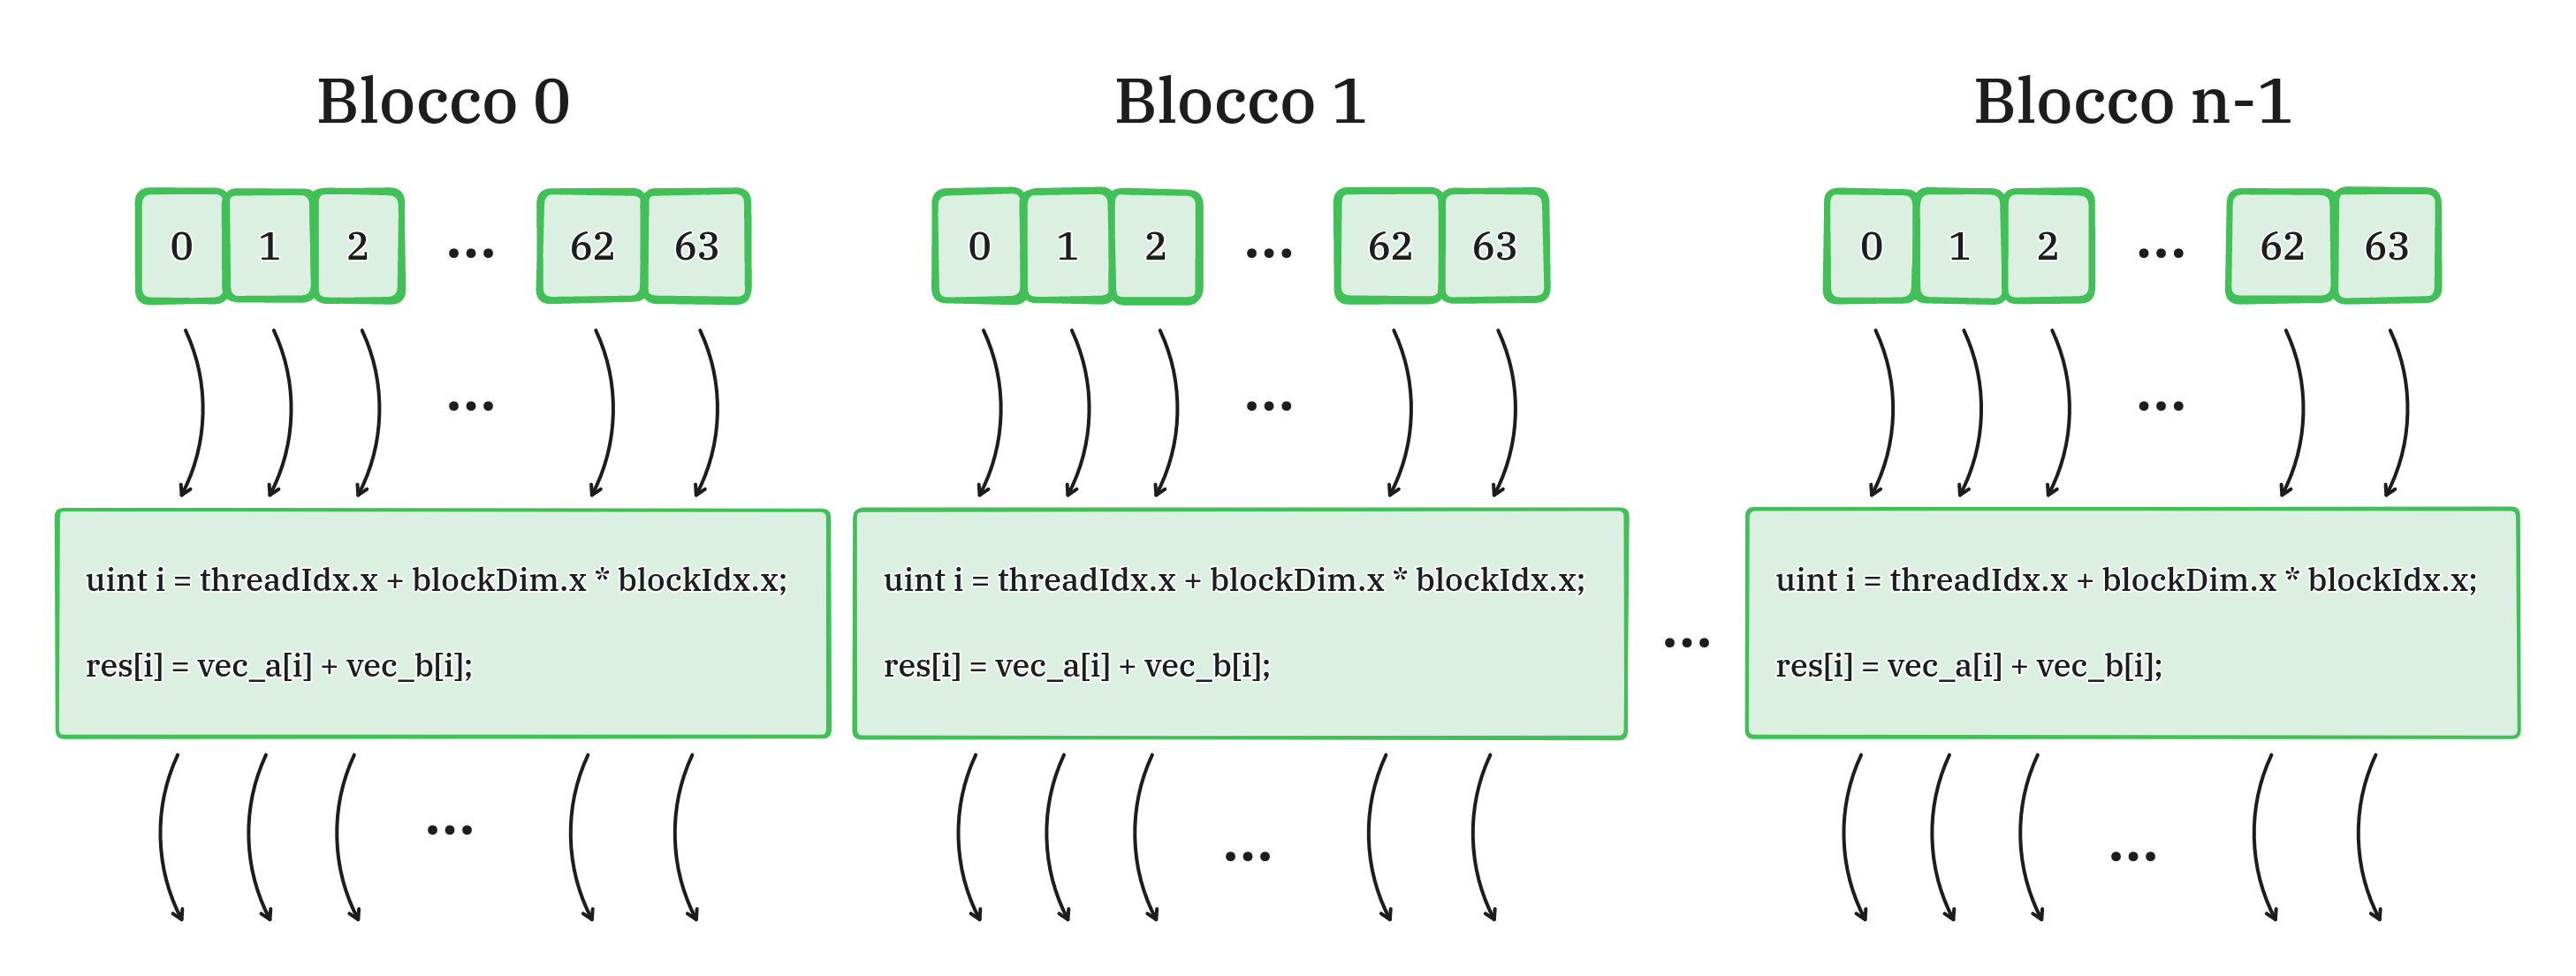
\includegraphics[width=.9\linewidth]{images/chapter2/grid.png}
    \caption{Esecuzione di programma CUDA}
    \label{fig:grid}
\end{figure}

Il codice kernel viene eseguito parallelamente da ogni thread della GPU seguendo il paradigma Single Program Multiple Data (\gls{SPMD}), che differisce dal SIMD per l'assenza del vincolo che ogni istruzione debba essere eseguita in contemporanea su ogni thread. Il singolo thread esegue tre operazioni: lettura dei dati dai vettori di input, somma dai dati e scrittura del dato sul vettore di output. Ogni thread esegue queste stesse identiche istruzioni, la differenza sta nelle aree di memoria su cui quelle esse vengono eseguite: \verb|uint i = threadIdx.x + blockDim.x * blockIdx.x| indica l'indice del vettore, e quindi l'aera di memoria sui cui lavorare, partendo dai parametri \verb|threadIdx|, \verb|blockDim| e \verb|blockIdx|. Come illustrato in fig \ref{fig:grid} la griglia sarà quindi composta da \verb|n| blocchi da 64 thread ciascuno, il numero effettivo dei blocchi dipende dalla lunghezza \verb|len| dei vettori, poiché si è deciso che 64 thread fissi devono essere presenti in ogni blocco.

\vspace{5mm}
\begin{lstlisting}[language=C++, caption=Kernel CUDA di somma di vettori, label=lis:sum_vec_kern]
__global__ void kernelFn(int *vec_a, int *vec_b, int *res, uint n) {
  uint i = threadIdx.x + blockDim.x * blockIdx.x;

  if (i < n) {
    res[i] = vec_a[i] + vec_b[i];
  }
}\end{lstlisting}
\vspace{5mm}

Il codice in \ref{lis:sum_vec_kern} è schematizzato in fig. \ref{fig:sum_vec}. Supponiamo adesso che la dimensione dei vettori sia 132, non multiplo di 64 (\verb|blockDim|). Il blocco condizionale \verb|if (i<n) {...}| indica che i thread nel blocco con \verb|blockIdx=2|, che si occuperanno di sommare gli elementi con indici \verb|i=128,129,130,131|, devono eseguire le operazioni solo se, appunto, \verb|i| è minore della lunghezza massima del vettore \verb|n|. Sebbene per questo specifico esempio non sia necessario al fine della corretta esecuzione del programma, è buona prassi aggiungere sempre questo tipo di condizione sui dati per evitare letture/scritture su aree di memoria non allocate.

\begin{figure}[ht]
    \centering
    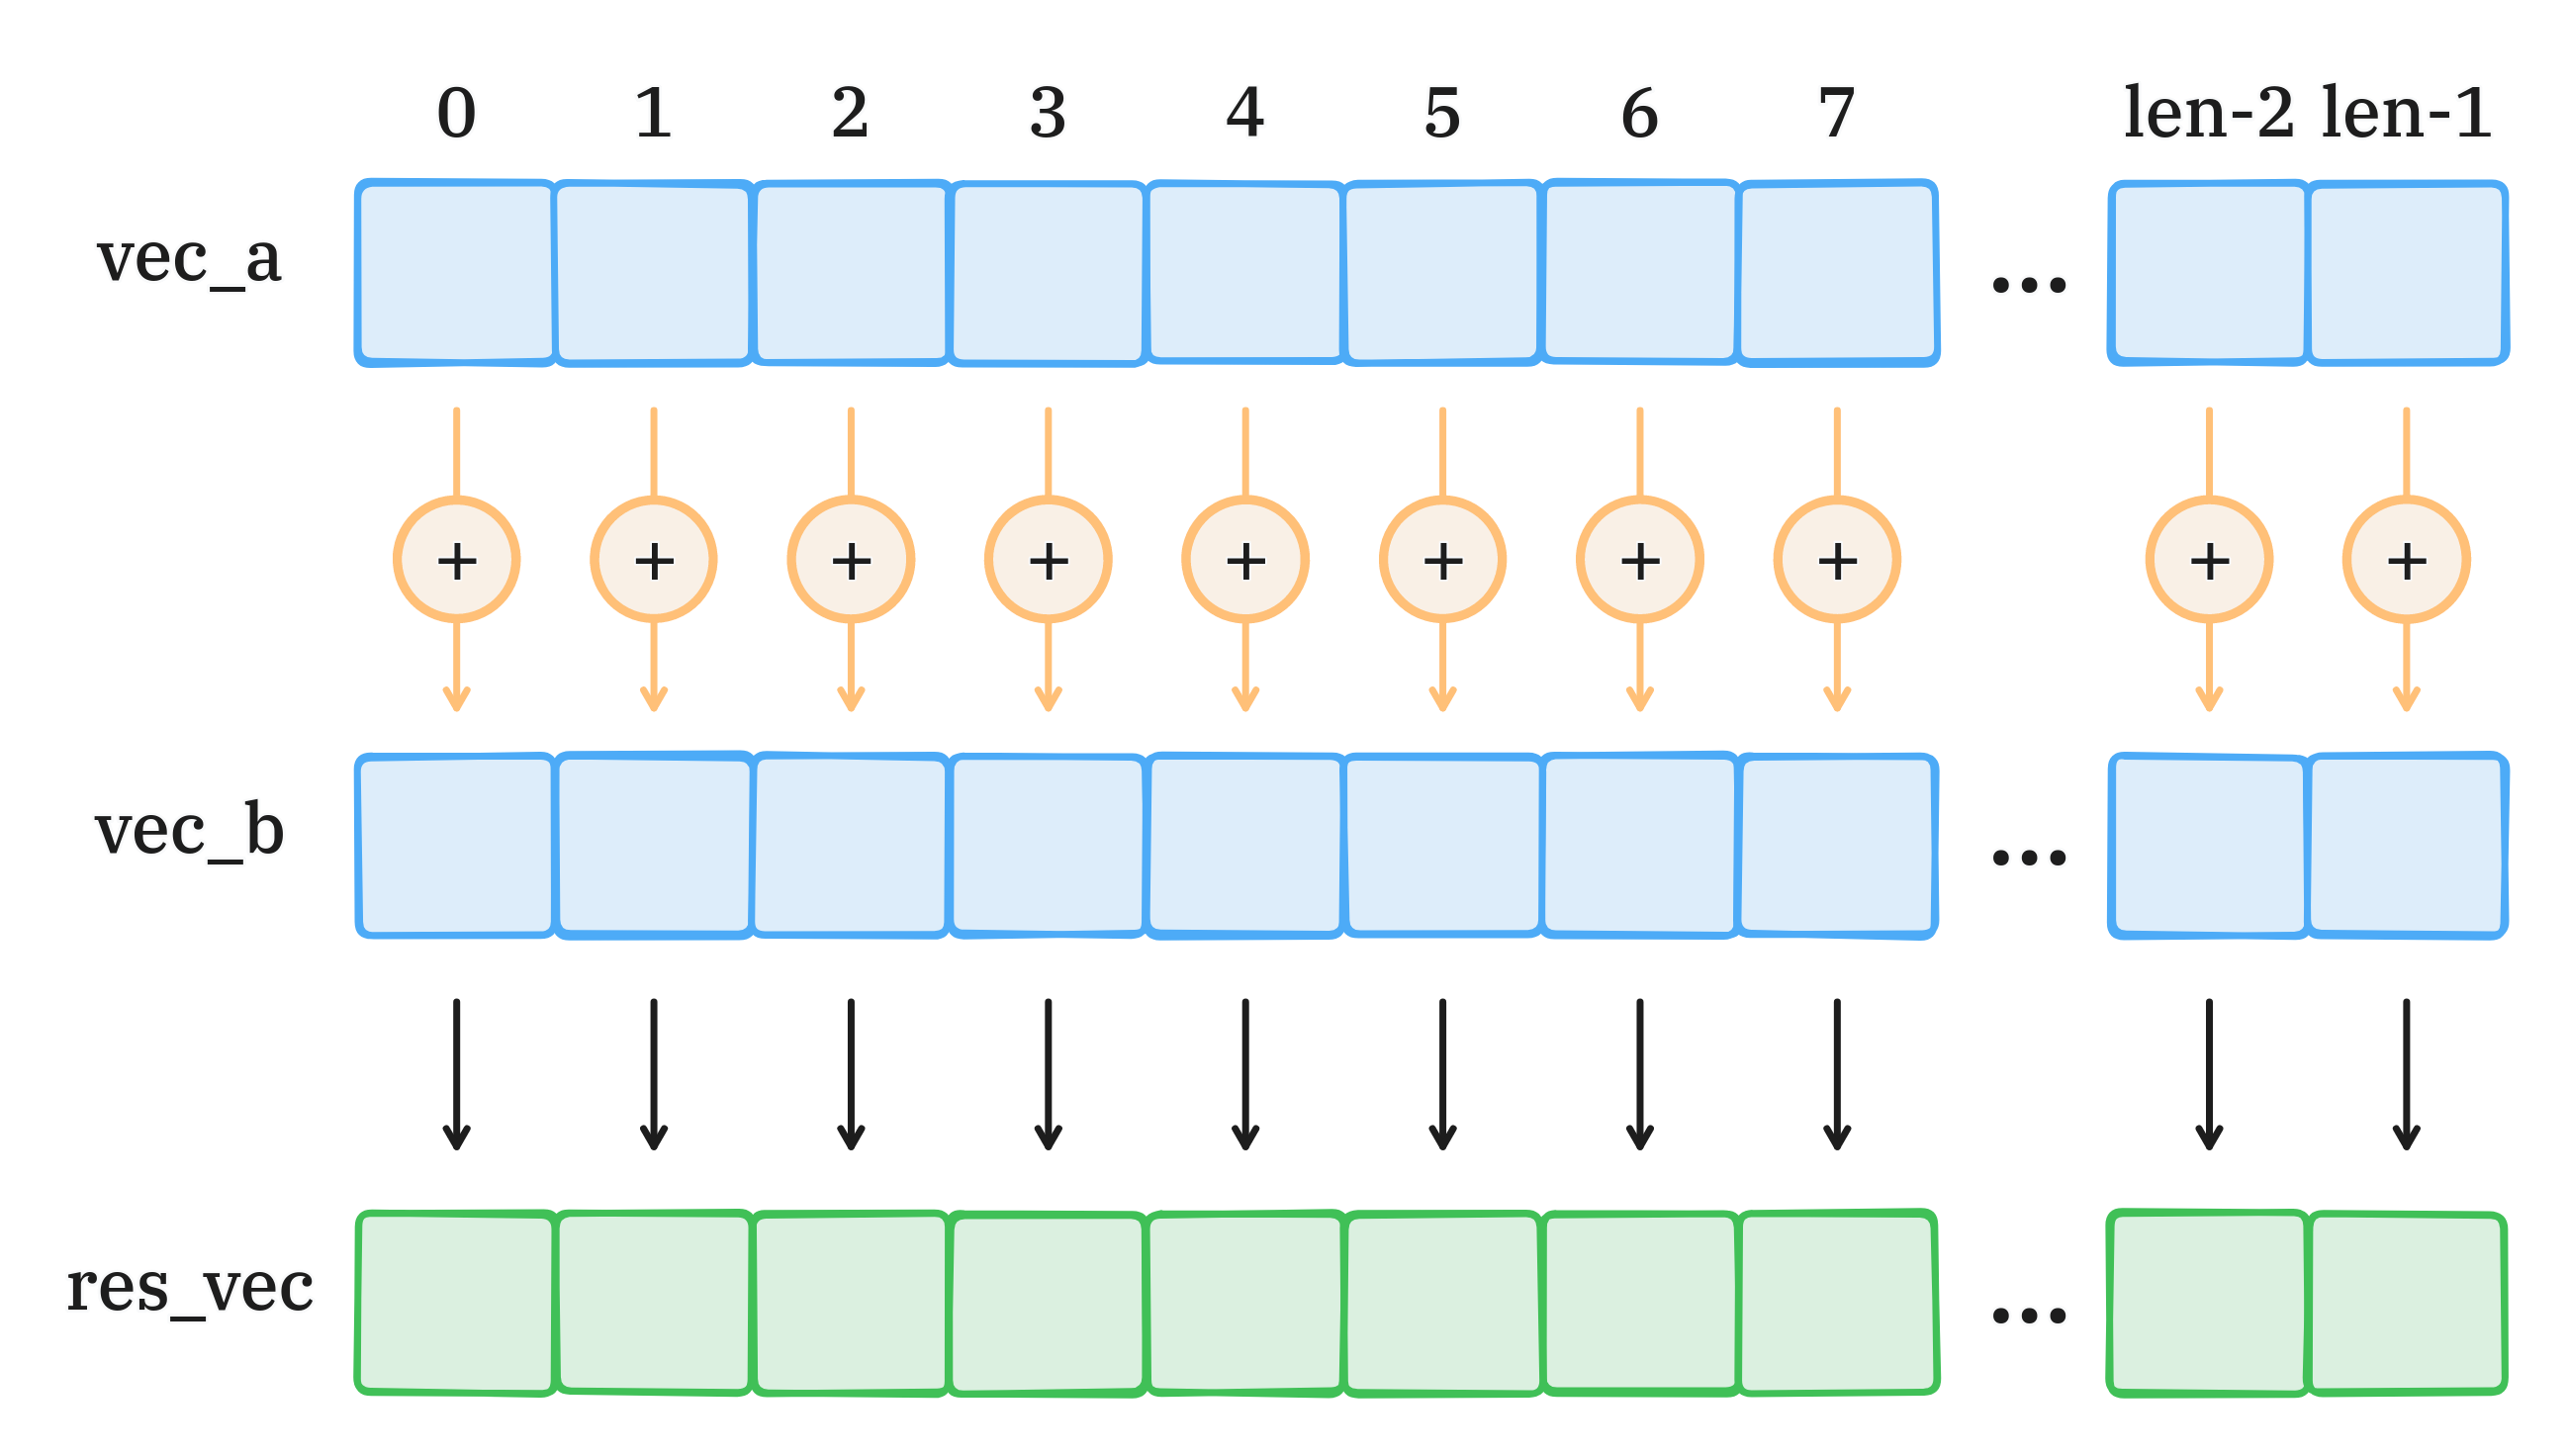
\includegraphics[width=.9\linewidth]{images/chapter2/sum_vec.png}
    \caption{Somma parallela di vettori}
    \label{fig:sum_vec}
\end{figure}

Come si è illustrato, in poco più di 30 righe di codice si è in grado di accelerare, in CUDA, una semplice operazione di somma di vettori. Nella prossima sezione si illustrerà lo stesso programma, ma utilizzando le API Vulkan tramite il linguaggio di programmazione Rust.

\subsection[Vulkan]{Vulkan}

Vulkan è una rivoluzionaria API per grafica e calcolo 3D ad alte prestazioni progettata per le moderne architetture a pipeline delle GPU, mantenendo il supporto multi-piattaforma tipico di OpenGL. Nonostante sia il successore dell'API OpenGL e OpenCL, è stato adottato un approccio completamente nuovo, per soddisfare le esigenze degli sviluppatori e lavorare in modo più efficiente con l'hardware della GPU. Vulkan è un'API esplicita, in grado di controllare le impostazioni dell'hardware per sfruttare al massimo la potenza del calcolo parallelo, sia in ambito grafico che di computing. Il driver layer è minimale e pone maggiori responsabilità sul programmatore dell'applicazione, che deve gestire le risorse, la gestione della memoria, la sincronizzazione, oltre all'applicazione stessa. Questa natura esplicita di Vulkan lo rende particolarmente verboso, soprattutto se confrontato a CUDA.

\begin{figure}[ht]
    \centering
    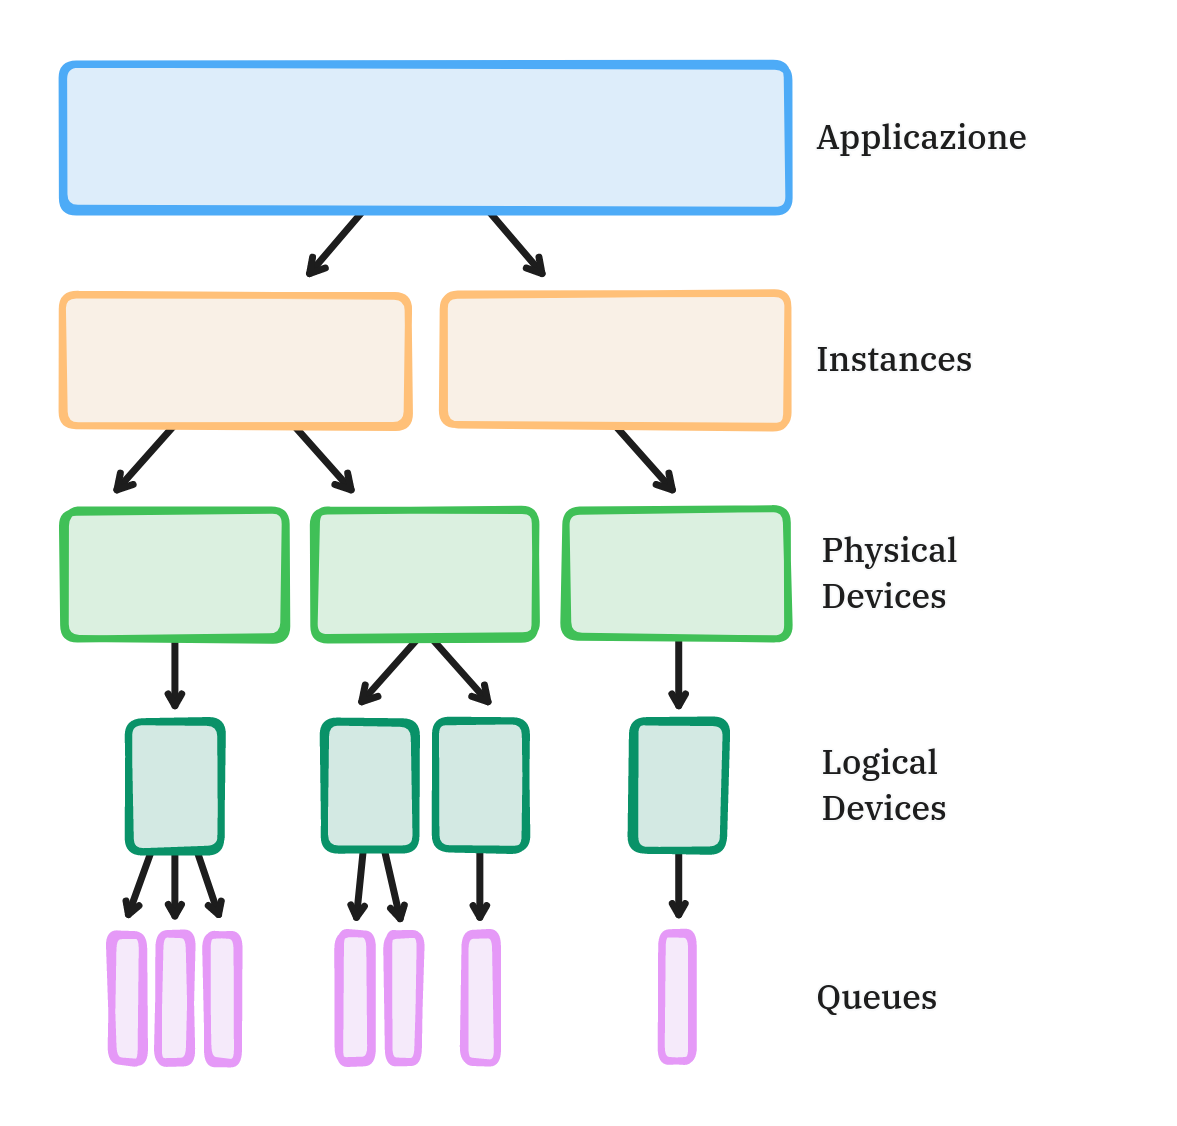
\includegraphics[width=.9\linewidth]{images/chapter2/vulkan_scheme.png}
    \caption{Schema di un'applicazione Vulkan}
    \label{fig:vulkan_scheme}
\end{figure}

In fig. \ref{fig:vulkan_scheme} è mostrato lo schema logico di un'applicazione Vulkan. 
Per scrivere un'applicazione Vulkan, per prima cosa va creata una \textit{instance}, che ha il compito di inizializzare la libreria Vulkan installata nel sistema e tenere traccia dello stato dell'applicazione. Una volta completata questa fase, si recuperano le informazioni sui \textit{physical device} disponibili nel sistema: si possono selezionare uno o più device. Per \textit{physical device} si intende l'hardware (CPU o GPU) su cui l'applicazione può essere eseguita. Se il nostro sistema dispone di molti \textit{physical device}, dato che ogni device ha determinate proprietà, si selezioneranno solo i device adatti all'applicazione. Un \textit{physical device} ha molte \textit{queue} che sono categorizzate in gruppi chiamati \textit{queue family}, in base alle loro proprietà. Ogni \textit{queue family} supporta una o più operazioni, ad esempio grafiche, di calcolo o di trasferimento di memoria. Poiché lo scopo di questo elaborato è sviluppare un'applicazione per il computing, verrà utilizzato un device appartenente alle \textit{queue family} ``computing'', che quindi supporta operazioni di calcolo. Una volta selezionato il device è necessario creare un \textit{logical device}, astrazione logica che rappresenta le connessioni al \textit{physical device} ed è usato dall'applicazione per interagire con l'hardware del dispositivo. Si possono anche creare più \textit{logical device} per lo stesso \textit{physical device}. Come ultima cosa, deve essere creata una \textit{queue}, della famiglia che ci interessa, a cui verrà sottoposto il carico di lavoro.

Sebbene le API Vulkan rilasciate da Khronos Group siano scritte in C++, esistono vari bindings per altri linguaggi. Come si è già accennato, in questo lavoro verrà usata la libreria Vulkano \cite[]{github:Vulkano} in Rust, in particolare al versione v0.33. Vulkano espone tutte le strutture dati necessarie per scrivere un'applicazione Vulkan, implementando il pattern \gls{RAII} e gestendo i riferimenti in memoria in safe Rust; questo permetterà di concentrarsi maggiormente sulla logica del programma piuttosto che sulla gestione di riferimenti in memoria, che è affidata al borrow checker \cite[]{Rust:borrow_checker} del compilatore di Rust. I benefici dell'usare Rust piuttosto che un altro linguaggio di programmazione verranno elencati successivamente nella prossima sezione.

\vspace{5mm}
\lstinputlisting[language=Rust, caption=Inizializzazione di Vulkan in Rust, label=lis:vulkan_init]{code/vulkan_init.rs} 
\vspace{5mm}

L'inizializzazione dell'applicazione Vulkan è illustrata in \ref{lis:vulkan_init}, nello specifico le variabili \verb|device| e \verb|queue| rappresentano, rispettivamente, il \textit{logical device} e la \textit{queue} su cui sottomettere il lavoro. 

In Vulkan il codice eseguito dalla GPU viene chiamato \textit{shader}, ed è scritto in \gls{GLSL}. Il linguaggio GLSL nasce come linguaggio di shading di OpenGL ed ha una sintassi simile al C e CUDA. Come illustrato in \ref{lis:vulkan_shader} i vettori di input, il vettore risultate e il parametro \verb|n|, che indica la lunghezza dei vettori, sono passati in modo esplicito prima dell'esecuzione della funzione \verb|main|. Importante notare che per ogni vettore vi è un parametro \verb|binding|, che, come vedremo in seguito, indica la precisa zona di memoria che viene passata alla GPU. Nella funzione \verb|main| possiamo notare similitudini con il kernel CUDA di \ref{lis:sum_vec_kern}, unica differenza degna di nota è il parametro che indica l'indice del vettore su cui eseguire le operazioni, in questo caso indicato con \verb|uint i = gl_GlobalInvocationID.x| piuttosto che sommando e moltiplicando manualmente indice di blocco e di thread, come avviene con CUDA.

\vspace{5mm}
\begin{lstlisting}[language=GLSL, caption=Shader GLSL di somma di vettori, label=lis:vulkan_shader]
#version 450

layout(local_size_x = 64, local_size_y = 1, local_size_z = 1) in;

layout(set = 0, binding = 0) readonly buffer VecA {
    int data[];
} vec_a;

layout(set = 0, binding = 1) readonly buffer VecB {
    int data[];
} vec_b;

layout(set = 0, binding = 2) writeonly buffer VecRes {
    int data[];
} res;

layout(push_constant) uniform PushConstants {
    uint n;
};

void main() {
    uint i = gl_GlobalInvocationID.x;

    if (i < n){
        res.data[i] = vec_a.data[i] + vec_b.data[i];
    }
}    
\end{lstlisting}
\vspace{5mm}

Il codice GLSL deve poi essere compilato in SPIR-V e infine caricato in memoria dall'applicazione Vulkan, con altre informazioni sui dettagli sull'esecuzione del codice. Questo meccanismo è illustrato in fig. \ref{fig:shader}. Passare per una rappresentazione binaria intermedia quale SPIR-V permette a Vulkan di avere supporto multi-piattaforma, lasciando ai driver del sistema del device i dettagli implementati su come eseguire il codice generato.

\begin{figure}[ht]
    \centering
    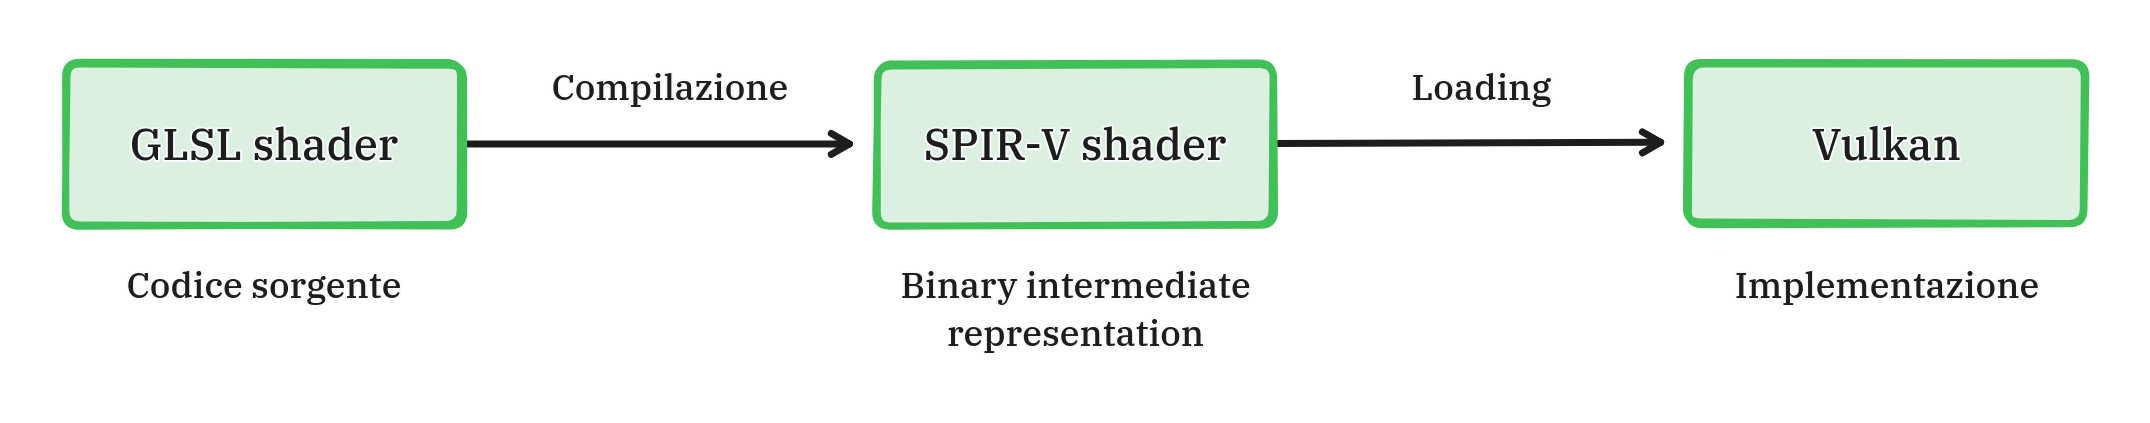
\includegraphics[width=.9\linewidth]{images/chapter2/shader.png}
    \caption{Generazione di uno shader SPIR-V e binding nell'applicazione Vulkan}
    \label{fig:shader}
\end{figure}

Per compilare e linkare lo shader, la liberia Vulkano fornisce delle macro, illustrate in \ref{lis:rust_macro}, che rendono tutto il processo automatico, agendo in fase di compilazione dell'eseguibile finale.

\newpage

\vspace{5mm}
\begin{lstlisting}[language=Rust, caption=Compilazione e binding dello shader GLSL, label=lis:rust_macro]
pub mod vec_sum {
    vulkano_shaders::shader! {
        ty: "compute",
        path: "vec_sum.glsl"
    }
}    
\end{lstlisting}
\vspace{5mm}

Una volta che Vulkan è inizializzata e lo shader è pronto per essere compilato, rimane solo allocare le risorse per l'implementazione del programma. Prima di addentrasi nei dettagli implementativi serve capire come Vulkan alloca e gestisce la memoria.


In Vulkan, considereremo due tipi di memoria: \textit{host memory} e \textit{device memory} schematizzate in fig. \ref{fig:host_device_mem}. La principale differenza tra le due è che la memoria host è accessibile e utilizzata dalla CPU, mentre la memoria device è accessibile solo dal dispositivo in cui viene eseguito lo shader. La memoria del dispositivo può avere alcune proprietà e tipi \cite[]{KG:VulkanGuide}. Ad esempio, un tipo di memoria può essere \verb|HOST_VISIBLE|, il che specifica che la memoria può essere mappata nello spazio di memoria dell'host e a cui si può accedere come se fosse memoria RAM; oppure può essere \verb|DEVICE_LOCAL| che indica che la memoria è, appunto, mappata nella memoria device. L'applicazione è responsabile dell'allocazione della memoria con il tipo appropriato in base alle esigenze. Vulkan offre questa flessibilità per migliorare le prestazioni e l'utilizzo della memoria \cite[]{KG:MemoryFlag}.

\begin{figure}[ht]
    \centering
    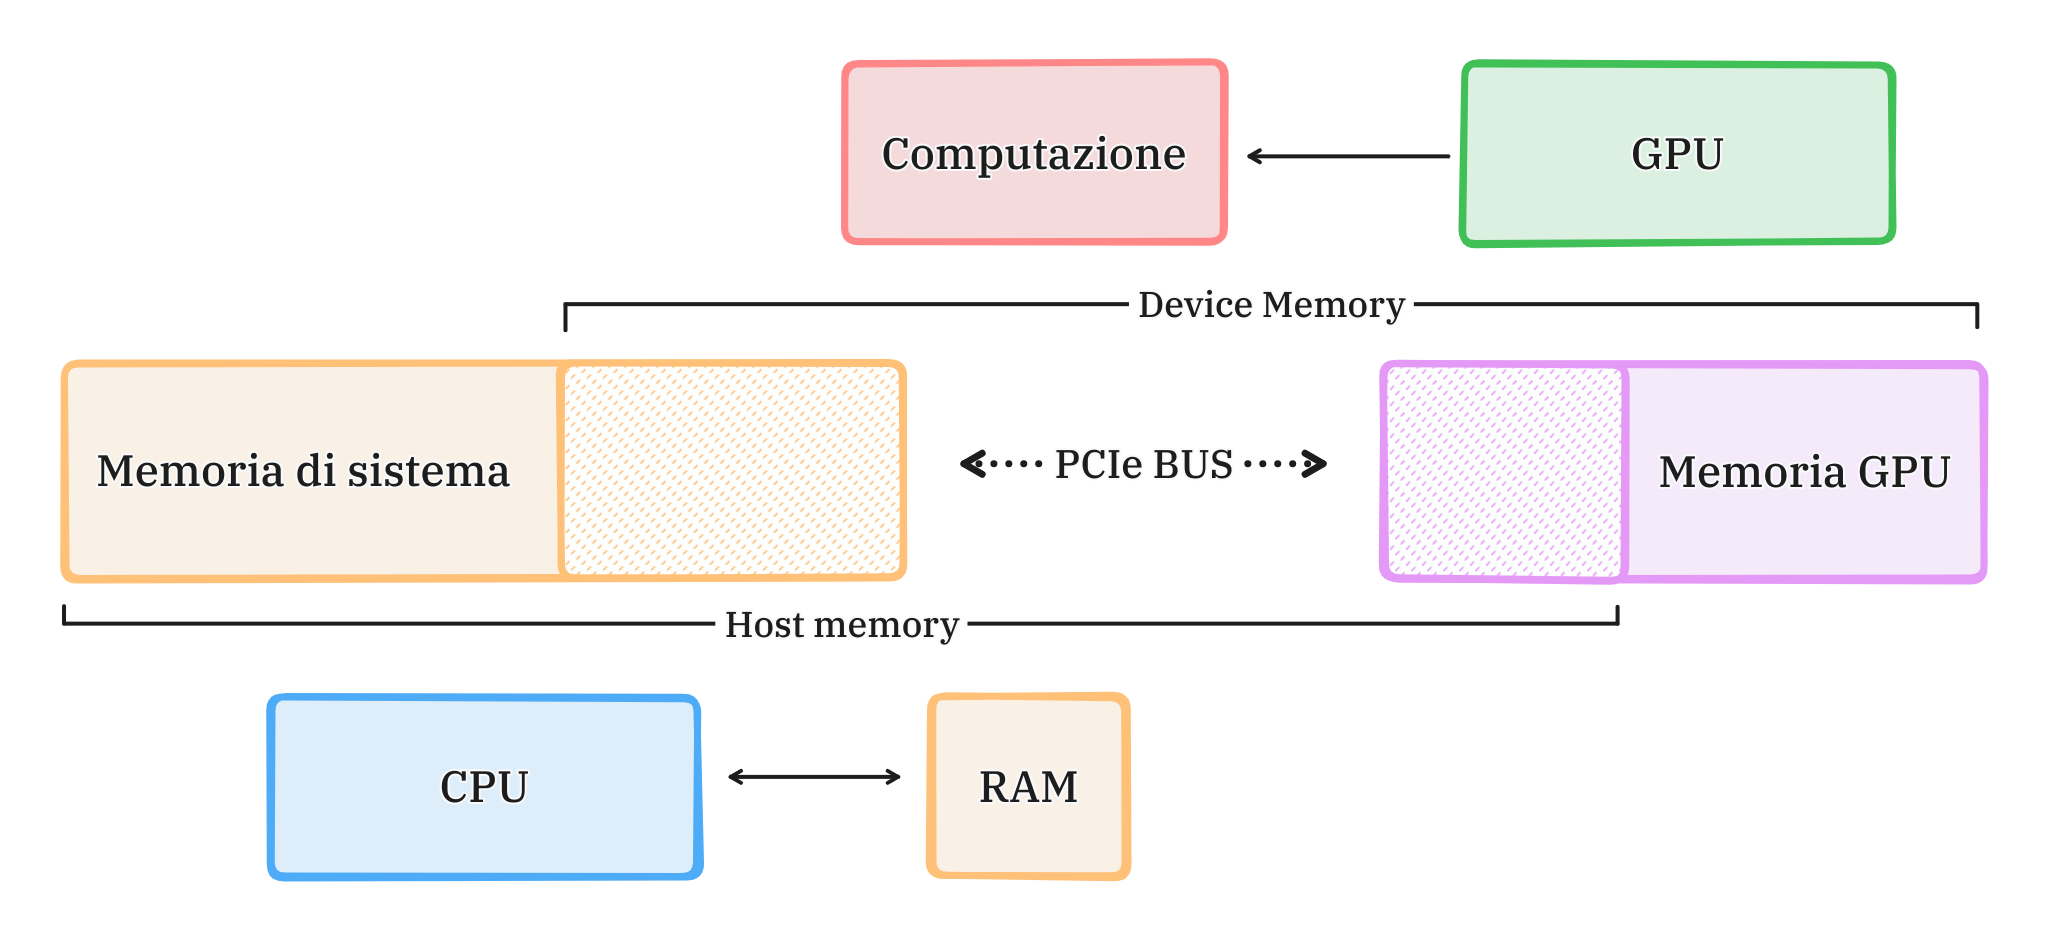
\includegraphics[width=.9\linewidth]{images/chapter2/host_device_mem.png}
    \caption{Memoria Host e Device}
    \label{fig:host_device_mem}
\end{figure}

Nella libreria Vulkano per indicare l'uso che si farà della memoria si utilizzano gli \verb|enum|: i primi due buffer infatti vengono marcati come \verb|MemoryUsage::Upload| poiché vengo inizializzati nell'host e trasferiti in memoria device, mentre il terzo buffer viene marcato come \verb|MemoryUsage::Download| perché appunto viene scritto dal device e letto dall'host. Il risultato è che tutti i buffer sono visibili sia dall'host che dal device, ma, mentre i primi due sono scrivibili solo dall'host, il terzo è scrivibili solo dal device. Queste politiche di accesso in memoria non solo permettono di isolare meglio i componenti ed evitare errori di programmazione, ma permettono anche ottimizzazioni da parte del compilatore SPIR-V per un'esecuzione più performante da parte del driver della GPU.

Nello shader in \ref{lis:vulkan_shader} i tre buffer vengono inizializzati con parametri che rispecchiano la natura e l'uso della memoria dalla prospettiva del device: i primi due vengono indicati col parametro \verb|readonly|, mentre il terzo con \verb|writeonly|. 

\vspace{5mm}
\begin{lstlisting}[language=Rust, caption=Inizializzazione buffer Vulkan, label=lis:vulkan_buffer]
let vec_a = Vec::new();
let vec_b = Vec::new();

let memory_allocator = StandardMemoryAllocator::new_default(device.clone());
let command_buffer_allocator =
    StandardCommandBufferAllocator::new(device.clone(), Default::default());

let buf_a = Buffer::from_iter(
    &memory_allocator,
    BufferCreateInfo {
        usage: BufferUsage::STORAGE_BUFFER,
        ..Default::default()
    },
    AllocationCreateInfo {
        usage: MemoryUsage::Upload,
        ..Default::default()
    },
    vec_a.iter(),
);
let buf_b = Buffer::from_iter(
    &memory_allocator,
    BufferCreateInfo {
        usage: BufferUsage::STORAGE_BUFFER,
        ..Default::default()
    },
    AllocationCreateInfo {
        usage: MemoryUsage::Upload,
        ..Default::default()
    },
    vec_b.iter(),
);
let buf_res = Buffer::new_slice(
    &memory_allocator,
    BufferCreateInfo {
        usage: BufferUsage::STORAGE_BUFFER,
        ..Default::default()
    },
    AllocationCreateInfo {
        usage: MemoryUsage::Download,
        ..Default::default()
    },
    len as u64,
)?;
\end{lstlisting}
\vspace{5mm}

Marcare tutti i tre vettori come \verb|HOST_VISIBLE| è necessario poiché i primi due di input sono inizializzati dalla CPU in memoria host, mentre l'ultimo viene letto dalla CPU per conoscere il risultato dell'operazione. In caso di computazioni intermedie, in cui non è necessario conoscere il risultato dell'operazione preliminare, ma soltanto passare il buffer a un altro shader per la computazione successiva, allora avrebbe senso marcare l'area di memoria come \verb|DEVICE_LOCAL| (utilizzando \verb|MemoryUsage::DeviceOnly|) evitando così overhead da eventuali accessi in memoria di sistema.

\begin{figure}[ht]
    \centering
    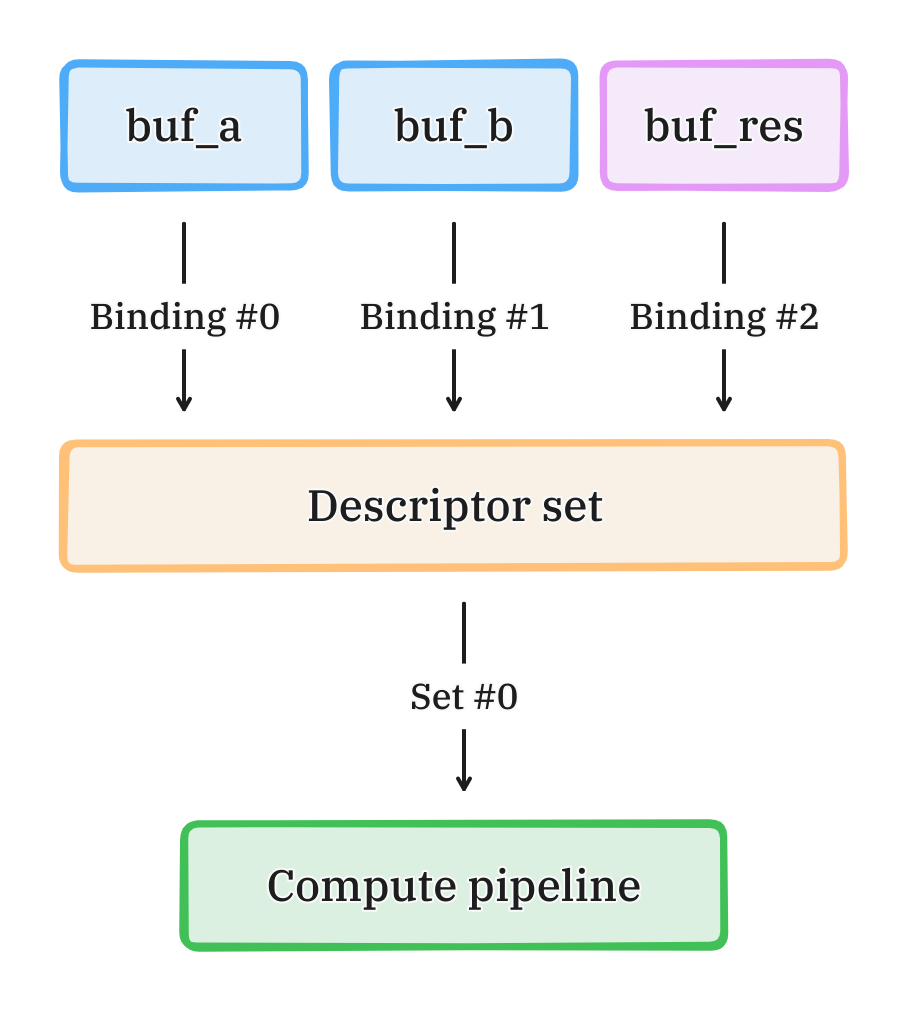
\includegraphics[width=.5\linewidth]{images/chapter2/pipeline.png}
    \caption{Descriptor set e compute pipeline}
    \label{fig:vulkan_pipeline}
\end{figure}

Dopo aver inizializzato i buffer bisogna creare dei \textit{descriptor set} che servono a specificare e gestire i dati di input e output per il kernel di calcolo. Questi vengono passati alla \textit{compute pipeline}, che definisce il flusso di operazioni parallele che vengono eseguite sui dati durante il processo di calcolo. In  fig. \ref{fig:vulkan_pipeline} è illustrata l'inizializzazione del \textit{descriptor set} e della \textit{compute pipeline}.

\newpage 

\vspace{5mm}
\begin{lstlisting}[language=Rust, caption=Inizializzazione della compute pipeline, label=lis:vulkan_pipeline]
let descriptor_set_allocator = 
    StandardDescriptorSetAllocator::new(device.clone());

let shader = loader::vec_sum::load(device)?;
let pipeline = ComputePipeline::new(
    device.clone(),
    shader
        .entry_point("main")
        .ok_or(anyhow!("No entry point in shader"))?,
    &(),
    None,
    |_| {},
)?;
let layout = pipeline.layout.set_layouts().get(0).unwrap();
let set = PersistentDescriptorSet::new(
    &descriptor_set_allocator,
    layout.clone(),
    [
        WriteDescriptorSet::buffer(0, buf_a),
        WriteDescriptorSet::buffer(1, buf_b),
        WriteDescriptorSet::buffer(2, buf_res.clone()),
    ],
)?;
\end{lstlisting}
\vspace{5mm}

In ultimo, si deve allocare un \textit{command buffer} per definire e inviare le operazioni da eseguire sul device. Il \textit{command buffer} attiva la pipeline di calcolo, impostando i parametri e l'invio dei dati di input, includendo comandi per la sincronizzazione tra le diverse operazioni. Utilizzando il \textit{command buffer} in modo efficiente è possibile ottimizzare le prestazioni del calcolo parallelo, ad esempio raggruppando le operazioni correlate in un unico buffer e inviandole in blocco al device GPU.

\vspace{5mm}
\begin{lstlisting}[language=Rust, caption=Command buffer e dispatch, label=lis:vulkan_dispatch]
let push_constants = PushConstants { n: len as u32 };

let mut command_buffer_builder = AutoCommandBufferBuilder::primary(
    &command_buffer_allocator,
    queue.queue_family_index(),
    CommandBufferUsage::OneTimeSubmit,
)?;
command_buffer_builder
    .bind_pipeline_compute(pipeline.clone())
    .bind_descriptor_sets(
        PipelineBindPoint::Compute,
        pipeline.layout().clone(),
        0,
        set,
    )
    .push_constants(pipeline.layout().clone(), 0, push_constants)
    .dispatch([len as u32 / 64, 1, 1])?;
let command_buffer = command_buffer_builder.build()?;

let future = sync::now(device.clone())
    .then_execute(queue.clone(), command_buffer)?
    .then_signal_fence_and_flush()?;
future.wait(None)?;

let vec_res = buf_res.to_vec();

...
\end{lstlisting}
\vspace{5mm}

Come si evince dal codice, questa versione è molto più prolissa, della corrispettiva in CUDA. Il programmatore ha sì modo di avere più controllo sulle risorse del sistema, ma quando si devono eseguire shader semplici, categoria in cui ricadono la maggior parte di quelli per il computing, questo potrebbe essere un ostacolo alla scrittura di codice leggibile e mantenibile. Come già accennato in precedenza, si è utilizzato la libreria Vulkano che permette di scrivere l'applicazione in Rust, se si fosse scelto di scrivere l'applicazione con C++ avremmo avuto codice ancora più verboso, per via dell'allocazione manuale della memoria, e sicuramente più prono ad errori, dato che la gestione della memoria sarebbe stata affidata interamente al programmatore. In questo Rust è venuto in aiuto, gestendo tutte le risorse col paradigma RAII e permettendoci di concentrarci sulla logica applicativa. Nel prossimo capitolo verrà spiegata come  Rust gestisce la memoria e perché risulta più facile scrivere codice con elevato grado di correttezza e manutenibilità.

\section[Rust]{Rust}

Rust è un linguaggio di programmazione di sistema progettato con un focus sulla sicurezza, sulla concorrenza e sulle prestazioni. In particolare l'obiettivo primario del linguaggio è permettere la gestione della memoria in modo automatico, ma senza ricorrere a garbage collector o contatori di riferimenti. 

Gli errori di memoria sono oggi una delle principali cause di vulnerabilità nel software \cite[]{Mic:memory_safety}, causando disagi agli utenti e soprattutto perdite economiche per aziende. Rust mitiga questo problema incorporando funzionalità avanzate che forniscono sicurezza della memoria senza compromettere le prestazioni. Al centro della strategia di gestione della memoria di Rust ci sono le semantica di ownership e il borrow checker \cite[]{Rust:borrow_checker}, che lavorano insieme per produrre codice formalmente \textit{safe}. Il modello di ownership di Rust ruota attorno al concetto di ownership, dove ogni valore nel programma ha un unico owner in un dato momento. La deallocazione della memoria avviene quando le variabili escono fuori dallo scope, come avviene col paradigma RAII. Questo approccio deterministico elimina problemi come memory leaks e double free, comuni nei linguaggi intrinsecamente \textit{unsafe} come C e C++. Quando un valore viene assegnato a un'altra variabile o passato a una funzione, il possesso viene trasferito, garantendo che ci sia sempre un chiaro owner responsabile del rilascio della memoria. Inoltre, Rust utilizza le semantica di spostamento, impedendo l'uso accidentale di puntatori invalidati o riferimenti pendenti.

Il borrow checker è uno strumento di analisi statica integrato nel compilatore Rust che impone le regole che governano ownership e borrowing. Il borrowing consente a più riferimenti di accedere a un valore senza trasferire il possesso. Tuttavia, il borrow checker garantisce che questi riferimenti non sopravvivano al valore che prendono in prestito o provocano race condition dei dati. Rust supporta due tipi di borrowing: borrowing immutabile e mutabile. Il borrowing immutabile consente a più lettori di accedere a un valore contemporaneamente, mentre il borrowing mutabile garantisce l'accesso esclusivo, impedendo scritture concorrenti. Per facilitare il borrowing, Rust introduce il concetto di lifetimes, che tracciano la durata per cui i riferimenti sono validi. I lifetimes consentono al borrow checker di analizzare staticamente il codice e garantire che i riferimenti presi in prestito non sopravvivano ai valori a cui fanno riferimento.

\vspace{5mm}
\begin{lstlisting}[language=Rust, caption=Controllo dei puntatori in fase di compilazione, label=lis:rust_borrow_checker]
fn main(){
    let x = Vec::new();

    // y ora è l'owner del dato di y
    let y = x;

    drop(x); // errore di compilazione, y è l'owner

    let mut x = vec![1, 2, 3];
    let first = &x[0];

    // x viene spostato in y, first non è più valido
    let y = x;
    
    println!("{*first}"); // errore di compilazione
}
\end{lstlisting}
\vspace{5mm}

Il modello di ownership di Rust facilita la concorrenza sicura applicando regole rigorose sull'aliasing mutabile a tempo di compilazione. Rust garantisce che l'accesso concorrente ai dati condivisi sia privo di race condition, rendendo più facile scrivere codice concorrente corretto e scalabile.
Nonostante le sue forti garanzie sulla sicurezza, Rust offre prestazioni comparabili, e in alcuni casi migliori, rispetto a C e C++ \cite[]{Rust:bench}. Sfruttando ownership e borrowing per eliminare il sovraccarico a tempo di esecuzione associato alla garbage collection e ai controlli a runtime, Rust produce codice efficiente e di basso livello adatto alla programmazione di sistema e alle applicazioni critiche in termini di prestazioni.

\vspace{5mm}
\begin{lstlisting}[language=Rust, caption=Fearless concurrency, label=lis:rust_fearless_concurrency]
use std::rc::Rc; // reference counting
use std::sync::Arc; // atomic reference counting
use std::sync::Mutex; // mutable exclusion

fn main(){
    let rc = Rc::new("not thread safe");
    std::thread::spawn(move || {
        // errore di compilazione, Rc non implementa il trait Send
        println!("{:?}", rc); 
    });

    let arc = Arc::new("thread safe");
    std::thread::spawn(move || {
        // Arc implementa Send, quindi è thread safe
        println!("{:?}", arc);  // output: thread safe
    });

    let mut v = Vec::new();
    std::thread::spawn(move || {
        v.push(1); 
    });
    // errore di compilazione, accesso a v dopo il movimento
    println!("{:?}", v); 

    // Mutex permette l'accesso concorrente in mutua esclusione
    let v = Arc::new(Mutex::new(Vec::new())); 
    let arc_v = Arc::clone(&v);
    std::thread::spawn(move || {
        arc_v.lock().unwrap().push(1); 
    }).join().unwrap(); 

    println!("{:?}", *v.lock().unwrap()); // output: [1]
}
\end{lstlisting}
\vspace{5mm}

L'approccio innovativo di Rust alla gestione della memoria e alla sicurezza, offre significativi vantaggi rispetto ai linguaggi tradizionali di programmazione di sistema. Combinando sicurezza della memoria, concorrenza e prestazioni, Rust permette ai programmatori di scrivere software affidabile, efficiente e scalabile senza un enorme sforzo cognitivo. Inoltre Rust si posiziona da 8 anni come linguaggio più amato dagli sviluppatori \cite[]{Rust:love}, per il suo ecosistema ricco, i numerosi tool disponibili e la facilità con cui si riesce a produrre software efficiente e sicuro. L'esigenza di produrre codice sicuro, ma efficiente non è solo del settore privato, per massimizzare il ritorno di investimento nello sviluppo software; ma premura anche del settore pubblico, come dimostra il recente endorsement del governo USA per quanto riguarda la sicurezza del cyberspazio \cite[]{Gov:rust_use}. Rust ha tutte le premesse per ridefinire il panorama della programmazione di sistema per gli anni a venire e la scelta di usarlo, per questo tipo di applicazioni, si sposa bene con la natura verbosa di Vulkan. 